%%%%%
%
\section{Correction des fortes pr\'ecipitations mesur\'ees par pluviom\`etre (Algorithme de fortes pr\'ecipitations fourni par la
DSO)}

\itemstyle{Op\'erateur~:} \textsf{Correct\_fortes\_rr\_pluvio}
\index{Correct\_fortes\_rr\_pluvio}

%%%%%OBJET%%%%
\itemstyle{Objet~:}
Cet op�rateur corrige les �ventuels d�bordements non pris en compte par le pluviom\`etre en cas de fortes pr�cipitations. Le
cumul des intensit�s de pr�cipitation est major� en fonction de la valeur de l'intensit� par pas de 0.1 mm et le reste
est port� sur la mesure suivante.


%%%%%ARGUMENTS%%%%
\bigskip
%%%%%ENTREES%%%%
\begin{tabarg}
\multicolumn{3}{l}{\titretab {Entr\'ees}}\\
\hline
$RRB_{i}$ & Vecteur, {\tt float} & cumul des pr\'ecipitations sur une minute (mm)\\
$A$ & Coeff., \texttt{double} & Coefficient multiplicateur A du coefficient de correction Ki\\
$B$ & Coeff., \texttt{double} & Coefficient multiplicateur B du coefficient de correction Ki\\
$C$ & Coeff., {\tt double} & Coefficient C du coefficient de correction Ki.\\
$R$ & Coeff., {\tt double} & R�solution du pluviom\`etre.\\
\end{tabarg}

\medskip
%%%%%SORTIES%%%%
\begin{tabarg}
\multicolumn{3}{l}{\titretab {Sorties}}\\
\hline
$RRC_{i}$ & Vecteur, {\tt float[$Dim_{RRB_{i}}$]} & Cumul des pr\'ecipitations corrig\'ees(m�me unit\'e que $RRB_{i}$)\\
\end{tabarg}


%%%%%FORMULE%%%%
\itemstyle{Formule}

%Correct_fortes_rr_pluvio
%
%Algorithme utilis� :
%
%En entr�e :
%vecteur Mm	 Cumul des pr�cipitation minutes 
%A valeur du parametre de correction
%B  valeur du parametre de correction
%	m/s	 Vitesse du vent mesur�e par l'an�mom�tre associ�
%C  valeur du parametre de correction
%  	   	 R�sultat du comptage sup�rieur
%R  R�solution du pluviometre
%En sortie
%vecteur Mm	 Cumul corrig� des pr�cipitation minutes 
%

%Algorithme de traitement des fortes pr�cipitations:

Calcul de la correction \`a appliquer chaque minute i:

$I_i$: intensit� des pr�cipitations � la minute $i$ en mm 
$$
I_i = \left\lbrace
\begin{array}{ll}
0.7 & \text{ Si $I_i$ > 0.7 (250mm/h)}\\
RRB_i/60 & \text{ sinon} \\
\end{array}\\
\right.
$$

$K_i$: le coefficient de correction calcul� de la minute i\  :
$$K_i =  A \times I_i ^2 + B \times I_i +C$$

\begin{center}

\begin{figure}[htbp]
\centering
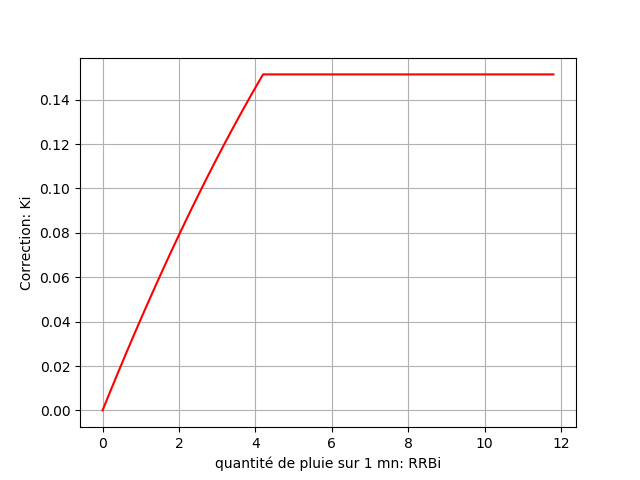
\includegraphics[scale=0.5]{./images/graph_formule_forte_pluie_K.png}
    \caption{Courbe de correction Ki en fonction de la quantit� de pluie par minute (pour un pluviom�tre pr�cis-m�canique 3070)}
\label{fig-formule}
\end{figure}
\end{center}

Et la Correction a appliquer a chaque minute $C_i$:
$$
C_i = K_i \times RRB_i
$$

Calcul de $RRC_i$: cumul des corrections � la minute $i$:

$$
RRC_i = RRB_i+INC_i
$$

$INC_i$ est la correction � appliquer au cumul des pr�cipitations \`a l'intant $i$ par pas de 0.1 mm. 
Si la correction $C_i$ n'atteint pas 0.1 mm, on garde le reste $RES_i$ en m�moire pour la minute suivante.
$RES_i$ est r�initialis� au bout de 2 minutes sans pluie.

$$
INC_i = \dfrac{\text{Partie Enti\`ere}  (10  \times ( Ci +RES_{i-1} ))}{10}
$$
$$
\text{et }  RES_i = \left\lbrace
\begin{array}{ll}
0 & \text{si } RRB_i = 0  \text{ et } RRB_{i-1} =0 \\
RES_{i-1}  + C_i  -INC_i & sinon \\
\end{array}\\
\right.
$$




%%%%%COMMENTAIRE%%%%
\itemstyle{Commentaire :}
Cette correction est utilis\'ee pour les pluvio pr�ci m�caniques du r�seau radome � la DSO.
\text{Valeurs des coefficients utilis�s pour le Pr\'ecis-m\'ecanique:}
$$
\begin{tabular}{lll}
A = -5.68 & B = 2.56 & C=0
\end{tabular}
$$



%%%%%AUTEUR%%%%

%%%%%AUTEUR%%%%
\itemstyle{Auteur~:}
CNRM/GMEI/TRAMM

%%%%%REFERENCE%%%%
\itemstyle{R\'ef\'erences~:}\\
Algorithme de traitement des donn\'ees du pr\'eci-M\'ecanique
Version 1.1 du 28/01/2013 DSO
